%!TEX root = ../report.tex

\chapter{State of the Art}

In the field of deep learning for computer vision, two distinct lines of research could be observed. One line of research includes the likes of ResNet, and Inception which push convolutional neural networks (CNN) deeper and wider. The focus here is to improve the accuracy on the task at hand. Another line of research is more concered with the practical use of deep learning in embedded or mobile devices. Here, approaches tend to focus on finding the best hyperparameters which require the least resources but yet perform with considerable accuracy. The range of approaches include attempts to design an resource efficient architecture by changing the number of layers and so on, attempts to compress CNNs using techniques like pruning, quantization and low-rank decomposition, and attempts to automatically search through the hyperparameter space to find the best hyperparameters by using reinforcement learning and evolutionary algorithms. 

In this chapter, we review networks which focus on improving accuracy (Section \ref{section:impacc}), and networks which focus on both accuracy and resource efficiency (Section \ref{section:acceff}) on the task of semantic segmentation. We also look into compression techniques called pruning and quantization in Section \ref{section:compress} and finally look into a method to generate datasets for semantic segmentation in Section \ref{section:dataset}.


\section{Improving accuracy}
\label{section:impacc}

In this section, we look into semantic segmentation networks which focus on improving accuracy. 

\subsection{Fully Convolutional Networks}

Fully Convolutional Networks \cite{DBLP:journals/corr/LongSD14} extend the success of convolutional neural networks on image classification, to the dense prediction task of semantic segmentation. Fully connected layers of image classification networks is converted to convolutional layers, which enables the prediction of a segmentation map and reduces computational cost as computation heavy fully connected layers are removed. Convolution and pooling layers downsample the input image to produce feature maps which have low spatial resolution. These feature maps are then upsamped using transposed convolution layers which use fractional stride which leads to increase in spatial resolution. Skip connections, as illustrated in Figure \ref{Fig:fcn} are used to coarse high layer information with fine low layer information to help refine the predicted segmentation map. 

	\begin{figure}
		\centering
		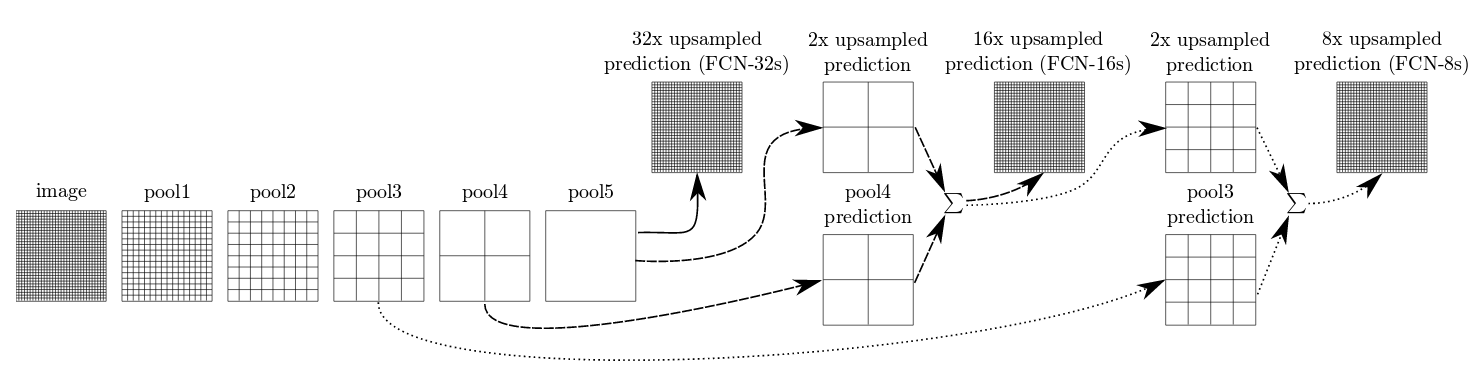
\includegraphics[width=1\linewidth]{images/fcn_skip}
		\caption{This figure illstrates the use of skip connections in Fully Convolutional Networks. Pooling layers downsample the input image. The pool5 layer results in 32 time reduction in spatial resolution of the input image. Three different predictions are shown. In the first, pool5 output is upsampled by 32. In the second, pool5 output is upsampled by 2, added with pool4 output with a skip connection and then upsampled by 16. In the third, pool5 output is upsampled by 2 two times, added with pool3 output using skip connection and then upsampled by 8. This third prediction is experimentally shown to produce finer predictions. }
		\label{Fig:fcn}
	\end{figure}

\subsection{Adversarial Networks}

\subsection{RGB-D data}

\subsection{Limited training data}

\section{Accuracy and resource efficiency}
\label{section:acceff}

In this section we look into semantic segmentation networks which consider both accuracy and resource efficiency in terms of memory and inference time. These approaches focus on reducing resource requirements and also improve accuracy.

\subsection{SegNet}

SegNet proposed the use of an encoder-decoder architecture for semantic segmentation. 

\subsection{ENet}

\subsection{ICNet}

\section{Compressing DCNNs}
\label{section:compress}

In this section, we look into approaches which compress Deep Convolutional Neural Networks (DCNN) by reducing the number of parameters or by using low precision calculations. The goal is to reduce resource requirements while retaining or incurring acceptable loss in accuracy.

\subsection{Deep Compression}

\subsection{Pruning CNNs}

\subsection{Quantizing CNNs}

\section{Dataset}
\label{section:dataset}

In this section, we look into an approach to creating dataset for the task of semantic segmentation.

\subsection{Cityscapes dataset}


